%\documentclass{standalone}
%\usepackage{tikz}
%\usetikzlibrary{patterns,plotmarks}
%\begin{document}
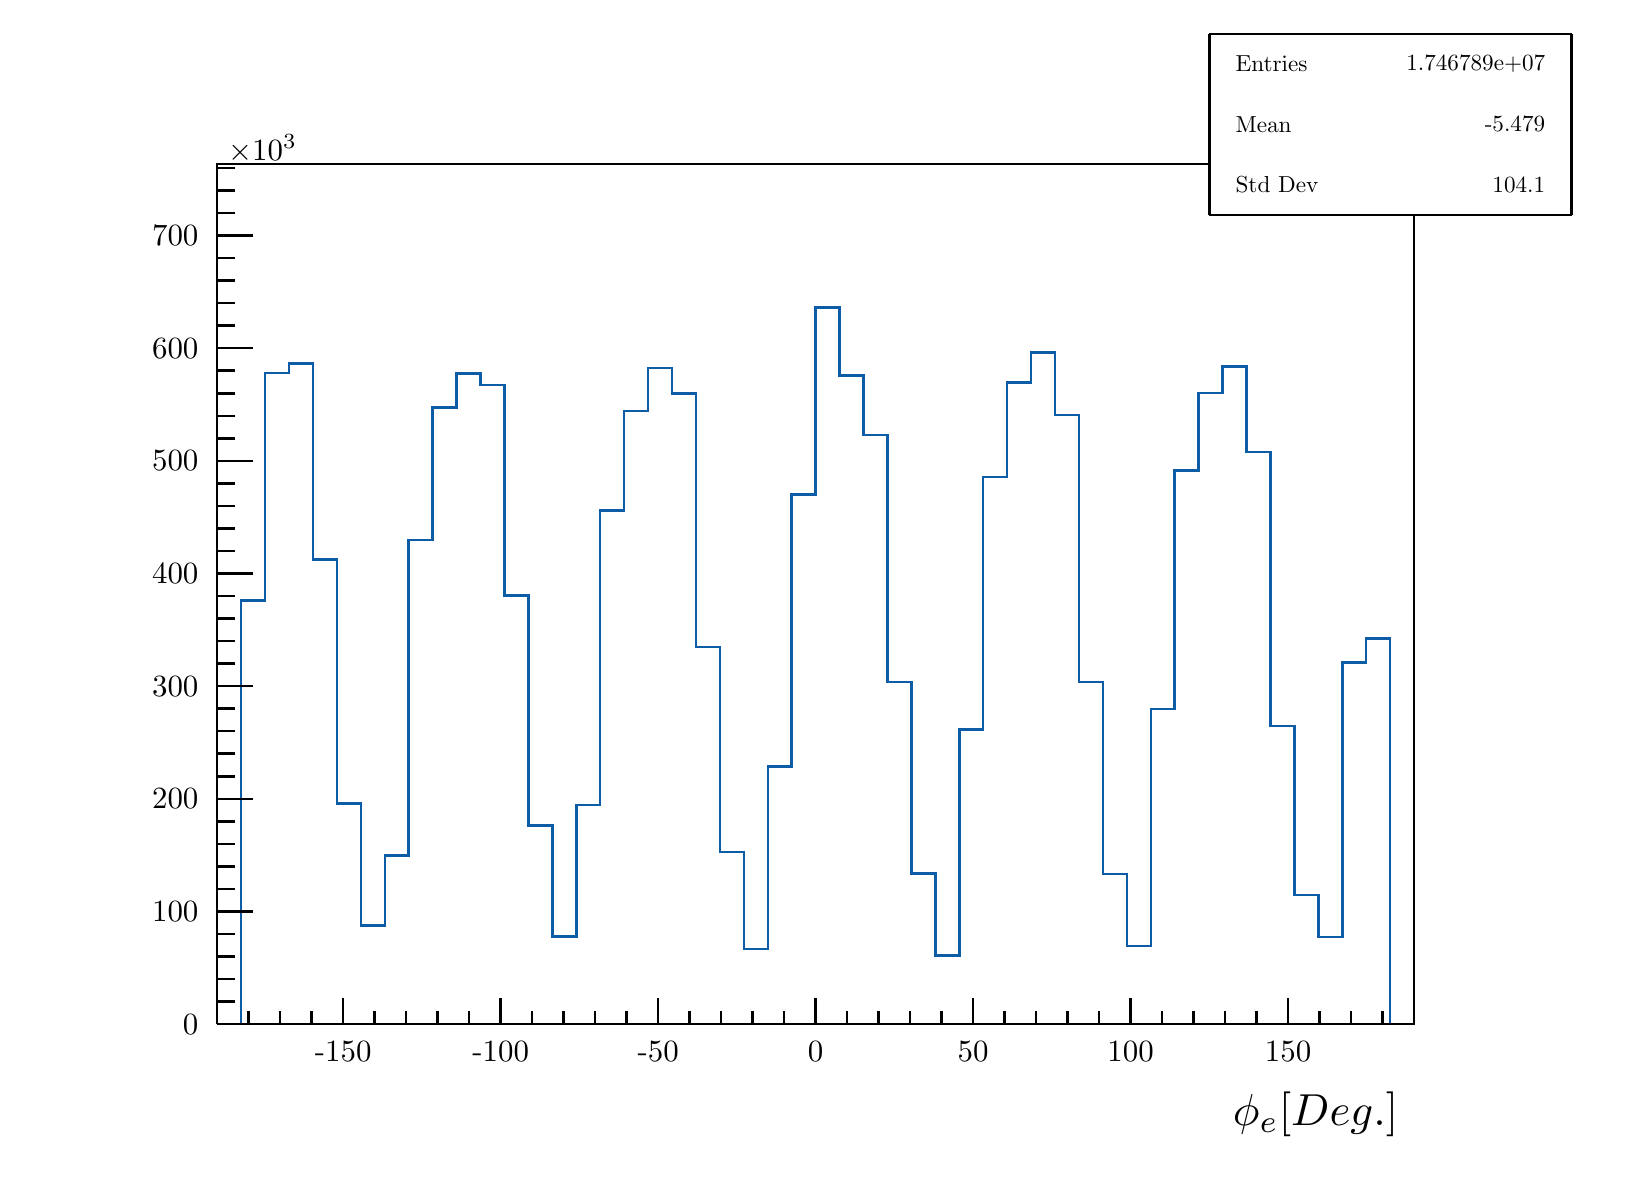
\begin{tikzpicture}
\def\CheckTikzLibraryLoaded#1{ \ifcsname tikz@library@#1@loaded\endcsname \else \PackageWarning{tikz}{usetikzlibrary{#1} is missing in the preamble.} \fi }
\CheckTikzLibraryLoaded{patterns}
\CheckTikzLibraryLoaded{plotmarks}
\pgfdeclareplotmark{cross} {
\pgfpathmoveto{\pgfpoint{-0.3\pgfplotmarksize}{\pgfplotmarksize}}
\pgfpathlineto{\pgfpoint{+0.3\pgfplotmarksize}{\pgfplotmarksize}}
\pgfpathlineto{\pgfpoint{+0.3\pgfplotmarksize}{0.3\pgfplotmarksize}}
\pgfpathlineto{\pgfpoint{+1\pgfplotmarksize}{0.3\pgfplotmarksize}}
\pgfpathlineto{\pgfpoint{+1\pgfplotmarksize}{-0.3\pgfplotmarksize}}
\pgfpathlineto{\pgfpoint{+0.3\pgfplotmarksize}{-0.3\pgfplotmarksize}}
\pgfpathlineto{\pgfpoint{+0.3\pgfplotmarksize}{-1.\pgfplotmarksize}}
\pgfpathlineto{\pgfpoint{-0.3\pgfplotmarksize}{-1.\pgfplotmarksize}}
\pgfpathlineto{\pgfpoint{-0.3\pgfplotmarksize}{-0.3\pgfplotmarksize}}
\pgfpathlineto{\pgfpoint{-1.\pgfplotmarksize}{-0.3\pgfplotmarksize}}
\pgfpathlineto{\pgfpoint{-1.\pgfplotmarksize}{0.3\pgfplotmarksize}}
\pgfpathlineto{\pgfpoint{-0.3\pgfplotmarksize}{0.3\pgfplotmarksize}}
\pgfpathclose
\pgfusepathqstroke
}
\pgfdeclareplotmark{cross*} {
\pgfpathmoveto{\pgfpoint{-0.3\pgfplotmarksize}{\pgfplotmarksize}}
\pgfpathlineto{\pgfpoint{+0.3\pgfplotmarksize}{\pgfplotmarksize}}
\pgfpathlineto{\pgfpoint{+0.3\pgfplotmarksize}{0.3\pgfplotmarksize}}
\pgfpathlineto{\pgfpoint{+1\pgfplotmarksize}{0.3\pgfplotmarksize}}
\pgfpathlineto{\pgfpoint{+1\pgfplotmarksize}{-0.3\pgfplotmarksize}}
\pgfpathlineto{\pgfpoint{+0.3\pgfplotmarksize}{-0.3\pgfplotmarksize}}
\pgfpathlineto{\pgfpoint{+0.3\pgfplotmarksize}{-1.\pgfplotmarksize}}
\pgfpathlineto{\pgfpoint{-0.3\pgfplotmarksize}{-1.\pgfplotmarksize}}
\pgfpathlineto{\pgfpoint{-0.3\pgfplotmarksize}{-0.3\pgfplotmarksize}}
\pgfpathlineto{\pgfpoint{-1.\pgfplotmarksize}{-0.3\pgfplotmarksize}}
\pgfpathlineto{\pgfpoint{-1.\pgfplotmarksize}{0.3\pgfplotmarksize}}
\pgfpathlineto{\pgfpoint{-0.3\pgfplotmarksize}{0.3\pgfplotmarksize}}
\pgfpathclose
\pgfusepathqfillstroke
}
\pgfdeclareplotmark{newstar} {
\pgfpathmoveto{\pgfqpoint{0pt}{\pgfplotmarksize}}
\pgfpathlineto{\pgfqpointpolar{44}{0.5\pgfplotmarksize}}
\pgfpathlineto{\pgfqpointpolar{18}{\pgfplotmarksize}}
\pgfpathlineto{\pgfqpointpolar{-20}{0.5\pgfplotmarksize}}
\pgfpathlineto{\pgfqpointpolar{-54}{\pgfplotmarksize}}
\pgfpathlineto{\pgfqpointpolar{-90}{0.5\pgfplotmarksize}}
\pgfpathlineto{\pgfqpointpolar{234}{\pgfplotmarksize}}
\pgfpathlineto{\pgfqpointpolar{198}{0.5\pgfplotmarksize}}
\pgfpathlineto{\pgfqpointpolar{162}{\pgfplotmarksize}}
\pgfpathlineto{\pgfqpointpolar{134}{0.5\pgfplotmarksize}}
\pgfpathclose
\pgfusepathqstroke
}
\pgfdeclareplotmark{newstar*} {
\pgfpathmoveto{\pgfqpoint{0pt}{\pgfplotmarksize}}
\pgfpathlineto{\pgfqpointpolar{44}{0.5\pgfplotmarksize}}
\pgfpathlineto{\pgfqpointpolar{18}{\pgfplotmarksize}}
\pgfpathlineto{\pgfqpointpolar{-20}{0.5\pgfplotmarksize}}
\pgfpathlineto{\pgfqpointpolar{-54}{\pgfplotmarksize}}
\pgfpathlineto{\pgfqpointpolar{-90}{0.5\pgfplotmarksize}}
\pgfpathlineto{\pgfqpointpolar{234}{\pgfplotmarksize}}
\pgfpathlineto{\pgfqpointpolar{198}{0.5\pgfplotmarksize}}
\pgfpathlineto{\pgfqpointpolar{162}{\pgfplotmarksize}}
\pgfpathlineto{\pgfqpointpolar{134}{0.5\pgfplotmarksize}}
\pgfpathclose
\pgfusepathqfillstroke
}
\definecolor{c}{rgb}{1,1,1};
\draw [color=c, fill=c] (0,0) rectangle (20,14.3719);
\draw [color=c, fill=c] (2.4,1.72462) rectangle (17.6,12.6472);
\definecolor{c}{rgb}{0,0,0};
\draw [c,line width=0.9] (2.4,1.72462) -- (2.4,12.6472) -- (17.6,12.6472) -- (17.6,1.72462) -- (2.4,1.72462);
\definecolor{c}{rgb}{1,1,1};
\draw [color=c, fill=c] (2.4,1.72462) rectangle (17.6,12.6472);
\definecolor{c}{rgb}{0,0,0};
\draw [c,line width=0.9] (2.4,1.72462) -- (2.4,12.6472) -- (17.6,12.6472) -- (17.6,1.72462) -- (2.4,1.72462);
\definecolor{c}{rgb}{0.0470588,0.364706,0.647059};
\draw [c,line width=0.9] (2.4,1.72462) -- (2.704,1.72462) -- (2.704,7.10349) -- (3.008,7.10349) -- (3.008,9.99062) -- (3.312,9.99062) -- (3.312,10.1156) -- (3.616,10.1156) -- (3.616,7.62163) -- (3.92,7.62163) -- (3.92,4.52773) -- (4.224,4.52773) --
 (4.224,2.97831) -- (4.528,2.97831) -- (4.528,3.8674) -- (4.832,3.8674) -- (4.832,7.86969) -- (5.136,7.86969) -- (5.136,9.55387) -- (5.44,9.55387) -- (5.44,9.98935) -- (5.744,9.98935) -- (5.744,9.83805) -- (6.048,9.83805) -- (6.048,7.16946) --
 (6.352,7.16946) -- (6.352,4.24344) -- (6.656,4.24344) -- (6.656,2.83829) -- (6.96,2.83829) -- (6.96,4.50569) -- (7.264,4.50569) -- (7.264,8.24669) -- (7.568,8.24669) -- (7.568,9.51341) -- (7.872,9.51341) -- (7.872,10.058) -- (8.176,10.058) --
 (8.176,9.72994) -- (8.48,9.72994) -- (8.48,6.51301) -- (8.784,6.51301) -- (8.784,3.90924) -- (9.088,3.90924) -- (9.088,2.67558) -- (9.392,2.67558) -- (9.392,4.99277) -- (9.696,4.99277) -- (9.696,8.45172) -- (10,8.45172) -- (10,10.8268) --
 (10.304,10.8268) -- (10.304,9.96201) -- (10.608,9.96201) -- (10.608,9.20812) -- (10.912,9.20812) -- (10.912,6.07078) -- (11.216,6.07078) -- (11.216,3.63779) -- (11.52,3.63779) -- (11.52,2.59535) -- (11.824,2.59535) -- (11.824,5.46776) --
 (12.128,5.46776) -- (12.128,8.66968) -- (12.432,8.66968) -- (12.432,9.87364) -- (12.736,9.87364) -- (12.736,10.2545) -- (13.04,10.2545) -- (13.04,9.45711) -- (13.344,9.45711) -- (13.344,6.06714) -- (13.648,6.06714) -- (13.648,3.6331) --
 (13.952,3.6331) -- (13.952,2.71376) -- (14.256,2.71376) -- (14.256,5.72431) -- (14.56,5.72431) -- (14.56,8.75767) -- (14.864,8.75767) -- (14.864,9.73887) -- (15.168,9.73887) -- (15.168,10.0769) -- (15.472,10.0769) -- (15.472,8.9929) --
 (15.776,8.9929) -- (15.776,5.50873) -- (16.08,5.50873) -- (16.08,3.36269) -- (16.384,3.36269) -- (16.384,2.83288) -- (16.688,2.83288) -- (16.688,6.31617) -- (16.992,6.31617) -- (16.992,6.61994) -- (17.296,6.61994) -- (17.296,1.72462) --
 (17.6,1.72462);
\definecolor{c}{rgb}{0,0,0};
\draw [c,line width=0.9] (2.4,1.72462) -- (17.6,1.72462);
\draw [c,line width=0.9] (4,2.0523) -- (4,1.72462);
\draw [c,line width=0.9] (4.4,1.88846) -- (4.4,1.72462);
\draw [c,line width=0.9] (4.8,1.88846) -- (4.8,1.72462);
\draw [c,line width=0.9] (5.2,1.88846) -- (5.2,1.72462);
\draw [c,line width=0.9] (5.6,1.88846) -- (5.6,1.72462);
\draw [c,line width=0.9] (6,2.0523) -- (6,1.72462);
\draw [c,line width=0.9] (6.4,1.88846) -- (6.4,1.72462);
\draw [c,line width=0.9] (6.8,1.88846) -- (6.8,1.72462);
\draw [c,line width=0.9] (7.2,1.88846) -- (7.2,1.72462);
\draw [c,line width=0.9] (7.6,1.88846) -- (7.6,1.72462);
\draw [c,line width=0.9] (8,2.0523) -- (8,1.72462);
\draw [c,line width=0.9] (8.4,1.88846) -- (8.4,1.72462);
\draw [c,line width=0.9] (8.8,1.88846) -- (8.8,1.72462);
\draw [c,line width=0.9] (9.2,1.88846) -- (9.2,1.72462);
\draw [c,line width=0.9] (9.6,1.88846) -- (9.6,1.72462);
\draw [c,line width=0.9] (10,2.0523) -- (10,1.72462);
\draw [c,line width=0.9] (10.4,1.88846) -- (10.4,1.72462);
\draw [c,line width=0.9] (10.8,1.88846) -- (10.8,1.72462);
\draw [c,line width=0.9] (11.2,1.88846) -- (11.2,1.72462);
\draw [c,line width=0.9] (11.6,1.88846) -- (11.6,1.72462);
\draw [c,line width=0.9] (12,2.0523) -- (12,1.72462);
\draw [c,line width=0.9] (12.4,1.88846) -- (12.4,1.72462);
\draw [c,line width=0.9] (12.8,1.88846) -- (12.8,1.72462);
\draw [c,line width=0.9] (13.2,1.88846) -- (13.2,1.72462);
\draw [c,line width=0.9] (13.6,1.88846) -- (13.6,1.72462);
\draw [c,line width=0.9] (14,2.0523) -- (14,1.72462);
\draw [c,line width=0.9] (14.4,1.88846) -- (14.4,1.72462);
\draw [c,line width=0.9] (14.8,1.88846) -- (14.8,1.72462);
\draw [c,line width=0.9] (15.2,1.88846) -- (15.2,1.72462);
\draw [c,line width=0.9] (15.6,1.88846) -- (15.6,1.72462);
\draw [c,line width=0.9] (16,2.0523) -- (16,1.72462);
\draw [c,line width=0.9] (4,2.0523) -- (4,1.72462);
\draw [c,line width=0.9] (3.6,1.88846) -- (3.6,1.72462);
\draw [c,line width=0.9] (3.2,1.88846) -- (3.2,1.72462);
\draw [c,line width=0.9] (2.8,1.88846) -- (2.8,1.72462);
\draw [c,line width=0.9] (2.4,1.88846) -- (2.4,1.72462);
\draw [c,line width=0.9] (16,2.0523) -- (16,1.72462);
\draw [c,line width=0.9] (16.4,1.88846) -- (16.4,1.72462);
\draw [c,line width=0.9] (16.8,1.88846) -- (16.8,1.72462);
\draw [c,line width=0.9] (17.2,1.88846) -- (17.2,1.72462);
\draw [anchor=base] (4,1.25035) node[scale=1.11607, color=c, rotate=0]{-150};
\draw [anchor=base] (6,1.25035) node[scale=1.11607, color=c, rotate=0]{-100};
\draw [anchor=base] (8,1.25035) node[scale=1.11607, color=c, rotate=0]{-50};
\draw [anchor=base] (10,1.25035) node[scale=1.11607, color=c, rotate=0]{0};
\draw [anchor=base] (12,1.25035) node[scale=1.11607, color=c, rotate=0]{50};
\draw [anchor=base] (14,1.25035) node[scale=1.11607, color=c, rotate=0]{100};
\draw [anchor=base] (16,1.25035) node[scale=1.11607, color=c, rotate=0]{150};
\draw [anchor= east] (17.6,0.574874) node[scale=1.61829, color=c, rotate=0]{$\phi_{e} [Deg.]$};
\draw [c,line width=0.9] (2.4,1.72462) -- (2.4,12.6472);
\draw [c,line width=0.9] (2.856,1.72462) -- (2.4,1.72462);
\draw [c,line width=0.9] (2.628,2.01074) -- (2.4,2.01074);
\draw [c,line width=0.9] (2.628,2.29685) -- (2.4,2.29685);
\draw [c,line width=0.9] (2.628,2.58296) -- (2.4,2.58296);
\draw [c,line width=0.9] (2.628,2.86908) -- (2.4,2.86908);
\draw [c,line width=0.9] (2.856,3.15519) -- (2.4,3.15519);
\draw [c,line width=0.9] (2.628,3.4413) -- (2.4,3.4413);
\draw [c,line width=0.9] (2.628,3.72742) -- (2.4,3.72742);
\draw [c,line width=0.9] (2.628,4.01353) -- (2.4,4.01353);
\draw [c,line width=0.9] (2.628,4.29964) -- (2.4,4.29964);
\draw [c,line width=0.9] (2.856,4.58576) -- (2.4,4.58576);
\draw [c,line width=0.9] (2.628,4.87187) -- (2.4,4.87187);
\draw [c,line width=0.9] (2.628,5.15798) -- (2.4,5.15798);
\draw [c,line width=0.9] (2.628,5.4441) -- (2.4,5.4441);
\draw [c,line width=0.9] (2.628,5.73021) -- (2.4,5.73021);
\draw [c,line width=0.9] (2.856,6.01632) -- (2.4,6.01632);
\draw [c,line width=0.9] (2.628,6.30243) -- (2.4,6.30243);
\draw [c,line width=0.9] (2.628,6.58855) -- (2.4,6.58855);
\draw [c,line width=0.9] (2.628,6.87466) -- (2.4,6.87466);
\draw [c,line width=0.9] (2.628,7.16077) -- (2.4,7.16077);
\draw [c,line width=0.9] (2.856,7.44689) -- (2.4,7.44689);
\draw [c,line width=0.9] (2.628,7.733) -- (2.4,7.733);
\draw [c,line width=0.9] (2.628,8.01911) -- (2.4,8.01911);
\draw [c,line width=0.9] (2.628,8.30523) -- (2.4,8.30523);
\draw [c,line width=0.9] (2.628,8.59134) -- (2.4,8.59134);
\draw [c,line width=0.9] (2.856,8.87745) -- (2.4,8.87745);
\draw [c,line width=0.9] (2.628,9.16357) -- (2.4,9.16357);
\draw [c,line width=0.9] (2.628,9.44968) -- (2.4,9.44968);
\draw [c,line width=0.9] (2.628,9.73579) -- (2.4,9.73579);
\draw [c,line width=0.9] (2.628,10.0219) -- (2.4,10.0219);
\draw [c,line width=0.9] (2.856,10.308) -- (2.4,10.308);
\draw [c,line width=0.9] (2.628,10.5941) -- (2.4,10.5941);
\draw [c,line width=0.9] (2.628,10.8802) -- (2.4,10.8802);
\draw [c,line width=0.9] (2.628,11.1664) -- (2.4,11.1664);
\draw [c,line width=0.9] (2.628,11.4525) -- (2.4,11.4525);
\draw [c,line width=0.9] (2.856,11.7386) -- (2.4,11.7386);
\draw [c,line width=0.9] (2.856,11.7386) -- (2.4,11.7386);
\draw [c,line width=0.9] (2.628,12.0247) -- (2.4,12.0247);
\draw [c,line width=0.9] (2.628,12.3108) -- (2.4,12.3108);
\draw [c,line width=0.9] (2.628,12.5969) -- (2.4,12.5969);
\draw [anchor= east] (2.3,1.72462) node[scale=1.11607, color=c, rotate=0]{0};
\draw [anchor= east] (2.3,3.15519) node[scale=1.11607, color=c, rotate=0]{100};
\draw [anchor= east] (2.3,4.58576) node[scale=1.11607, color=c, rotate=0]{200};
\draw [anchor= east] (2.3,6.01632) node[scale=1.11607, color=c, rotate=0]{300};
\draw [anchor= east] (2.3,7.44689) node[scale=1.11607, color=c, rotate=0]{400};
\draw [anchor= east] (2.3,8.87745) node[scale=1.11607, color=c, rotate=0]{500};
\draw [anchor= east] (2.3,10.308) node[scale=1.11607, color=c, rotate=0]{600};
\draw [anchor= east] (2.3,11.7386) node[scale=1.11607, color=c, rotate=0]{700};
\draw [anchor=base west] (2.4,12.6975) node[scale=1.11607, color=c, rotate=0]{$\times10^{3}$};
\definecolor{c}{rgb}{1,1,1};
\draw [color=c, fill=c] (15,12.0005) rectangle (19.6,14.3);
\definecolor{c}{rgb}{0,0,0};
\draw [c,line width=0.9] (15,12.0005) -- (19.6,12.0005);
\draw [c,line width=0.9] (19.6,12.0005) -- (19.6,14.3);
\draw [c,line width=0.9] (19.6,14.3) -- (15,14.3);
\draw [c,line width=0.9] (15,14.3) -- (15,12.0005);
\draw [anchor= west] (15.23,13.9168) node[scale=0.837049, color=c, rotate=0]{Entries };
\draw [anchor= east] (19.37,13.9168) node[scale=0.837049, color=c, rotate=0]{   1.746789e+07};
\draw [anchor= west] (15.23,13.1503) node[scale=0.837049, color=c, rotate=0]{Mean  };
\draw [anchor= east] (19.37,13.1503) node[scale=0.837049, color=c, rotate=0]{ -5.479};
\draw [anchor= west] (15.23,12.3838) node[scale=0.837049, color=c, rotate=0]{Std Dev   };
\draw [anchor= east] (19.37,12.3838) node[scale=0.837049, color=c, rotate=0]{  104.1};
\definecolor{c}{rgb}{1,1,1};
\draw [color=c, fill=c] (15,12.0005) rectangle (19.6,14.3);
\definecolor{c}{rgb}{0,0,0};
\draw [c,line width=0.9] (15,12.0005) -- (19.6,12.0005);
\draw [c,line width=0.9] (19.6,12.0005) -- (19.6,14.3);
\draw [c,line width=0.9] (19.6,14.3) -- (15,14.3);
\draw [c,line width=0.9] (15,14.3) -- (15,12.0005);
\draw [anchor= west] (15.23,13.9168) node[scale=0.837049, color=c, rotate=0]{Entries };
\draw [anchor= east] (19.37,13.9168) node[scale=0.837049, color=c, rotate=0]{   1.746789e+07};
\draw [anchor= west] (15.23,13.1503) node[scale=0.837049, color=c, rotate=0]{Mean  };
\draw [anchor= east] (19.37,13.1503) node[scale=0.837049, color=c, rotate=0]{ -5.479};
\draw [anchor= west] (15.23,12.3838) node[scale=0.837049, color=c, rotate=0]{Std Dev   };
\draw [anchor= east] (19.37,12.3838) node[scale=0.837049, color=c, rotate=0]{  104.1};
\end{tikzpicture}
%\end{document}
